\chapter{Electroweak Theory}
\label{chap:SM}

Developed in the 1960s, the Glashow–Weinberg–Salam theory of \ac{EW} interaction is regarded by many physicists as the cornerstone of the \ac{SM}. It successfully unified the weak interaction with electromagnetism and postulated the existence of several new particles, all of which were later confirmed by experiments. One of the most important aspects of this theory is the \ew~gauge symmetry, which is discussed in \autoref{sec:Gauge}. The \ew~ symmetry is spontaneously broken through the Higgs mechanism, which is discussed in \autoref{sec:Higgs}. Finally, flavor physics and its connection to the Yukawa interaction is discussed in \autoref{sec:Flavor}. 

\section{Gauge Theory}
\label{sec:Gauge}

Fundamental forces in the \ac{SM} are formulated under a principle known as gauge invariance, where Lagrangian is invariant under local transformations of gauge groups. Taking \ac{QED} as an example, the local symmetry for a Dirac fermion is,

\begin{equation}
\psi\rightarrow e^{i\alpha(x)}\psi,
\end{equation}

where $\alpha(x)$ is a space-time dependent phase angle, hence the name ''local transformation''. The gauge group associated to this symmetry is $U(1)_{EM}$, where the subscript is a shorthand expression for ``electromagnetism''. Under a local $U(1)_{EM}$ rotation, Equation~\ref{eq:Dirac} can be written as:

\begin{equation}
\begin{split}
\label{eq:QEDGauge}
\mathcal{L}&=-\frac{1}{4}F_{\mu\nu}F^{\mu\nu}+ie^{-i\alpha(x)}\bar{\psi}\gamma^{\mu}\partial_{\mu}e^{i\alpha(x)}\psi-m\bar{\psi}\psi-e\bar{\psi}\gamma^{\mu}(A_{\mu}+\delta A_{\mu})\psi\\
&=\mathcal{L}_{Dirac}-\bar{\psi}\gamma^{\mu}\psi\partial_{\mu}\alpha(x)-e\bar{\psi}\gamma^{\mu}\delta A_{\mu}\psi.
\end{split}
\end{equation}

The gauge invariance requires $\delta A_{\mu}=-\frac{1}{e}\partial_{\mu}\alpha(x)$. This means the photon field transforms as:

\begin{equation}
A_{\mu}\rightarrow A_{\mu}-\frac{1}{e}\partial_{\mu}\alpha(x).
\end{equation}

This behavior of the photon field under gauge transformation cancels out the gauge dependency of the free Dirac Lagrangian, which ensures the gauge invariance of the theory. Therefore, vector bosons such as photons also called gauge bosons, and the associated quantum fields are also known as gauge fields. The Dirac Lagrangian can be re-written as,

\begin{equation}
\label{eq:QEDCov}
\mathcal{L}=-\frac{1}{4}F_{\mu\nu}F^{\mu\nu}+i\bar{\psi}\gamma^{\mu}D_{\mu}\psi-m\bar{\psi}\psi,
\end{equation}

where $D_{\mu}=\partial_{\mu}+ieA_{\mu}$ is known as the gauge covariant derivative. 

The mass term associated to the photon field $\frac{1}{2}m^2A_{\mu}A^{\mu}$ is however not gauge invariant as

\begin{equation}
[A_{\mu}-\frac{1}{e}\partial_{\mu}\alpha(x)][A^{\mu}-\frac{1}{e}\partial^{\mu}\alpha(x)]\neq A_{\mu}A^{\mu}.
\end{equation}

Effectively, this means gauge bosons such as photons must be massless in a gauge invariant theory. As a consequence, a new mechanism, known as the Higgs mechanism, is needed to explain the origin of weak boson masses, which is discussed in the following chapter. 

It should be pointed out that gauge symmetry is not a symmetry of nature. Unlike global symmetry that corresponds conserved current~\cite{Noether1918}, gauge symmetry is not physical and can not be measured by experiments. Nevertheless, its existence is necessary to regulate the redundant degree of freedom in the Lagrangian~\cite{SCHWARTZ}. 

\ac{QED} is also known as an abelian gauge theory as the $U(1)$ group operation is commutative. Chinese physicist Yang Chen-Ning and his American colleague Robert Mills at BrookHaven first generalized the concept of gauge invariance to the non-abelian Lie group, proposing what's now known as the Yang-Mills theory in 1954~\cite{Yang:1954ek}. Shortly after this work, Yang and his colleague Tsung-Dao Lee suggested parity might be violated in the weak interaction~\cite{Lee:1956qn}, which was later confirmed by the legendary Wu experiment led by Chien-Shiung Wu~\cite{Wu:1957my}. 

Not long after the Wu experiment, physicists had understood that only left-handed fermions and right-handed anti-fermions are involved in weak charged-current interactions. Moreover, the very existence of weak charged-current forced physicists to consider the interaction between photons and weak mediators. This led to many problems in the weak theory, for example, the exchange of photons in $s$-channel $\textsf{e}^{+}\textsf{e}^{-}\rightarrow\textsf{W}^{+}\textsf{W}^{-}$ would result in divergence at high energy unless there is a new massive neutral particle that mediates the weak interaction. Hints of the weak neutral current and the interplay between electromagnetism and the weak interaction prompted the efforts by physicists to relate these two forces under the framework of non-abelian gauge theory in early 1960s. 

Since fermions with different chiral structures were understood to be treated differently by the weak interaction, it was 
imperative to apply different gauge transformations to left-handed and right-handed fermionic fields. Initial work toward unification was done by American physicist Sheldon Glashow, who proposed the \ew~symmetry in 1961~\cite{Glashow:1961tr}, where $L$ denotes left-handed fields, and Y refers to the quantum number for hypercharge. Under this framework, left-handed components of the Dirac fields are organized into $SU(2)_{L}$ doublet,

\begin{equation}
L_{L}^{j}=\begin{pmatrix}\upnu_{\ell}^{j}\\ \ell^{j}\end{pmatrix}_{L}, Q_{L}^{\prime j}=\begin{pmatrix}q^{\prime j}_{u}\\q^{\prime j}_{d}\end{pmatrix}_{L}, j=1, 2, 3,
\end{equation}

where $\upnu_{\ell}^{j}$, $\ell^{j}$, $q^{\prime j}_{u}$, and $q^{\prime j}_{d}$ correspond to Dirac fields of neutrino, charged-lepton, up-type quark, and down-type quark, respectively. The right-handed components of the Dirac fields are treated as $SU(2)_{L}$ singlet: $\ell_{R}^{j}, u_{R}^{\prime j}, d_{R}^{\prime j}$, where a neutrino term is missing as only left-handed neutrinos have been observed in nature. The index $j$ in both doublets and singlets runs over the fermion generations. The left-handed doublets carry $\frac{1}{2}$ weak isospin charge, denoted by $T$. The third component of $T$, denoted by $T_3$, is $\frac{1}{2}$ for neutrinos and up-type quarks, and -$\frac{1}{2}$ for charged-leptons and down-type quarks in the $SU(2)_{L}$ doublets. All right-handed singlets carries 0 weak isospin charge, which prevents them from participating in the weak interaction. 

The \ew~symmetry introduces the following local gauge transformations:

\begin{equation}
\begin{split}
&\Psi_{L}\rightarrow\textsf{exp}[i\hat{T}_{i}\alpha^{i}(x)+i\frac{\hat{Y}}{2}\beta(x)]\Psi_{L},\\
&\Psi_{R}\rightarrow\textsf{exp}[i\frac{\hat{Y}}{2}\beta(x)]\Psi_{R},
\end{split}
\end{equation}

where $\hat{T}_{i}$ and $\hat{Y}$ denotes generators of the $SU(2)_{L}$ and $U(1)_{Y}$ group, respectively. To preserve gauge invariance, two massless gauge fields $W_{\mu}$ and $B_{\mu}$ are introduced. The corresponding gauge covariant derivative can be written as

\begin{equation}
D_{\mu}=\partial_{\mu}-ig\hat{T}_{i}W_{\mu}^{i}-ig^{\prime}\hat{Y}B_{\mu},
\end{equation}

where $g$ and $g^{\prime}$ coupling strength of the $SU(2)$ and $U(1)$ gauge fields, respectively. A linear combination of the first and second component $W_{\mu}^{i}$ gives rise to the weak charge-current interactions observed in experiments:

\begin{equation}
W^{\pm}_{\mu}=\frac{1}{\sqrt{2}}(W^{1}_{\mu}\mp W^{2}_{\mu}),
\end{equation}

while neutral-current interactions can be constructed by the remaining fields:

\begin{equation}
\label{}
\begin{pmatrix}B_{\mu}\\W_{\mu}^{3}\end{pmatrix}=\begin{pmatrix}\cos\theta_{W}&-\sin\theta_{W}\\\sin\theta_{W}&\cos\theta_{W}\end{pmatrix}\begin{pmatrix}A_{\mu}\\Z_{\mu}\end{pmatrix},
\end{equation}

where $A_{\mu}$ and $Z_{\mu}$ corresponds to the photon and Z boson, respectively, and $g\sin\theta_{W}=g^{\prime}\cos\theta_{W}=e$. The free parameter $\theta_{W}$ is referred to as the week mixing angle, or Weinberg angle, which has to be measured experimentally.

The relation between electric charge, weak isospin, and hyperchage is given by the Gell-Mann-Nishijima formula~\cite{Nakano:1953zz,Gell-Mann:1956iqa}:

\begin{equation}
Q=\frac{Y}{2}+T_{3}.
\end{equation}

The preliminary version of the \ac{EW} theory developed by Glashow didn't collect very good reception initially as all gauge fields in this theory were massless due to gauge invariance. Luckily, physicists didn't have to wait for long as the mechanism proposed by American physicist P. W. Anderson~\cite{Anderson:1963pc} in the following year (1962) had quickly gained attention. Extending on Anderson's work, the theory of symmetry breaking and mass generation was published by Higgs and others in 1964~\cite{PhysRevLett.13.321,PhysRevLett.13.508,PhysRevLett.13.585}, which led to the eventual completion of the \ac{EW} theory in the following years~\cite{Salam:1964ry,Weinberg:1967tq}.

\section{Higgs Mechanism}
\label{sec:Higgs}

\begin{figure}[tbh!]
 \begin{center}
 \begin{tabular}{c}
 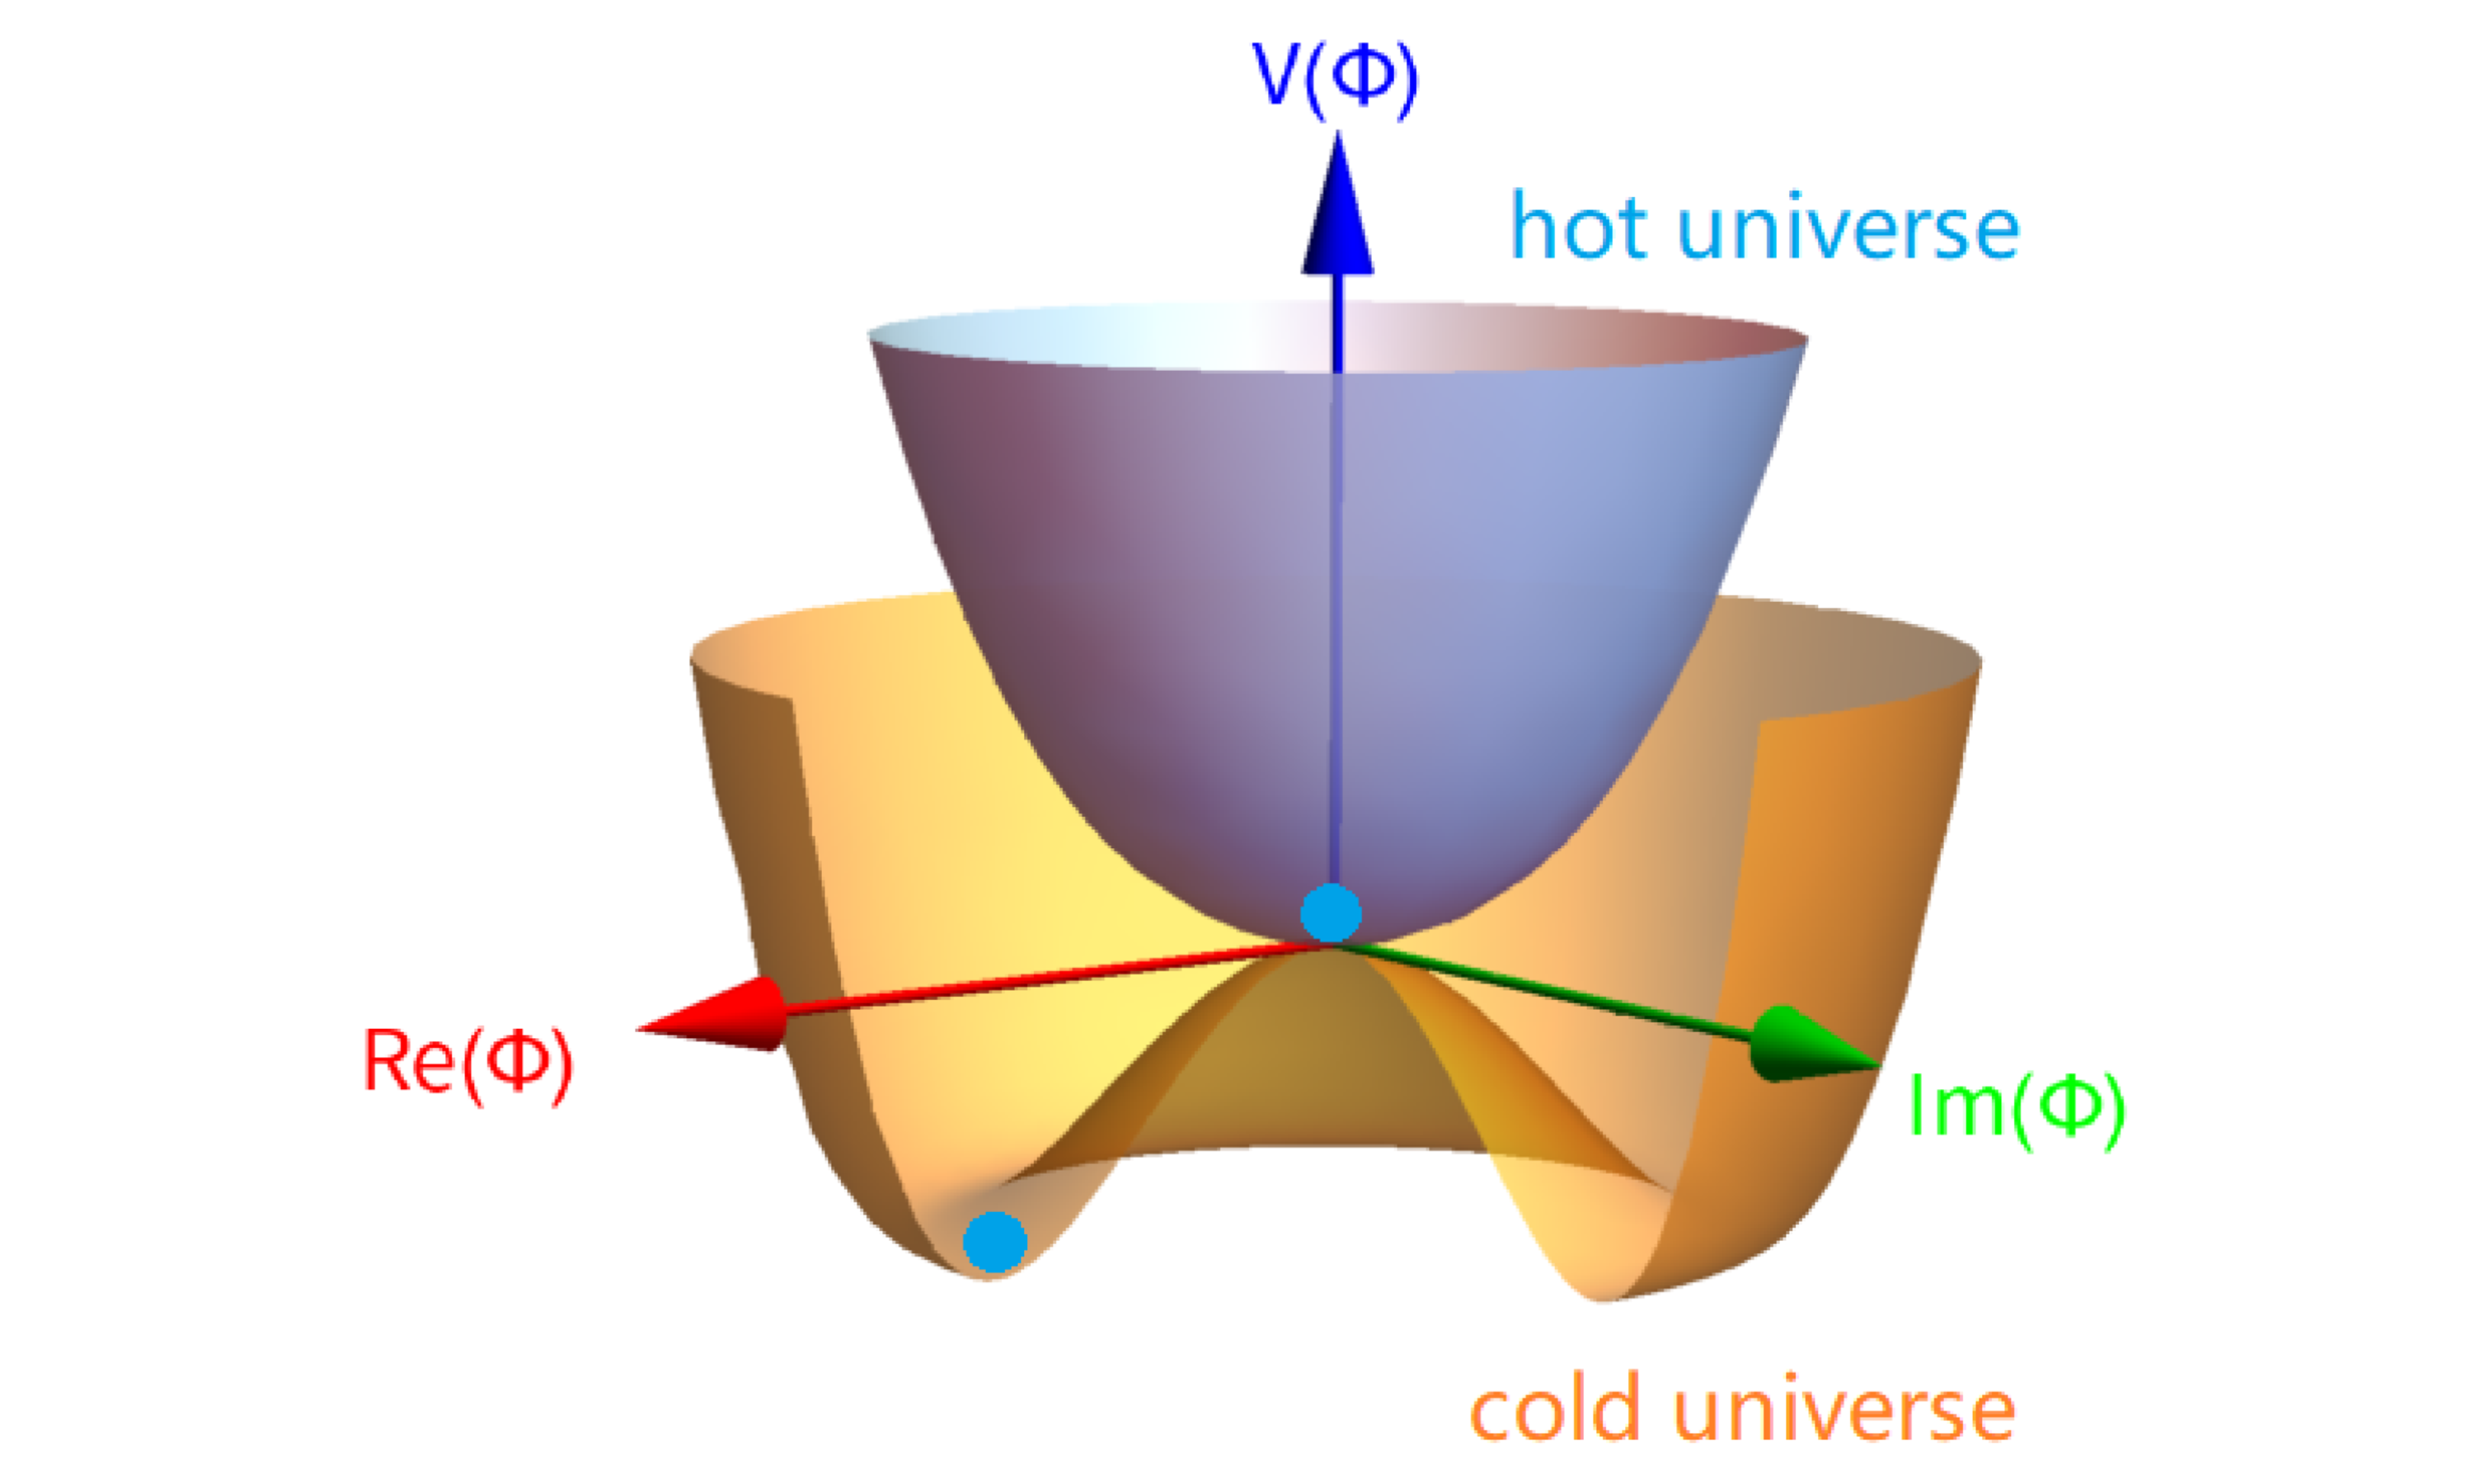
\includegraphics[width=0.7\textwidth]{figures/Part1/SM/HiggsPotential}
 \end{tabular}
 \caption{Possible shape of the Higgs potential before symmetry breaking in hot universe (blue) and after symmetry breaking in present universe (yellow).~\cite{universe9040178}}
 \label{fig:HiggsPotential}
 \end{center}
\end{figure}

\section{Flavor Sector}
\label{sec:Flavor}